\documentclass[11pt]{article}

\usepackage[margin=0.92in]{geometry}
\usepackage{amsmath,amssymb,amsthm,mathtools}
\usepackage{graphicx}
\usepackage[hidelinks]{hyperref}

\newtheorem{theorem}{Theorem}
\newtheorem{remark}{Remark}
\newcommand{\Cl}{\mathrm{Cl}_3^+}
\newcommand{\M}{\mathcal M^+}
\newcommand{\A}{\bigvee\!\M(B^3)}
\newcommand{\tr}{\operatorname{tr}}

\title{The Boundary Trace Algebra of Monogenic Spinors Need Not Be Isomorphic}
\author{Automated Math Discovery Candidate Counterexample}
\date{August 11, 2026}

\begin{document}
\maketitle

\begin{center}
\fbox{\parbox{0.92\textwidth}{\textbf{Status.}
Candidate full negative answer to open item (ii) in the further-results
section of arXiv:2203.00118, likely valid pending expert review.  On the
Euclidean unit three-ball, the algebra generated by monogenic spinor fields
contains the nonzero scalar field \(1-|x|^2\), whose boundary trace is zero.}}
\end{center}

\section*{Source Question}

Roberts asks whether the algebra generated by monogenic spinor fields and the
algebra generated by their boundary traces are isometrically isomorphic under
the trace map \cite{Roberts}.  The question is item (ii) on page 22:

\begin{center}
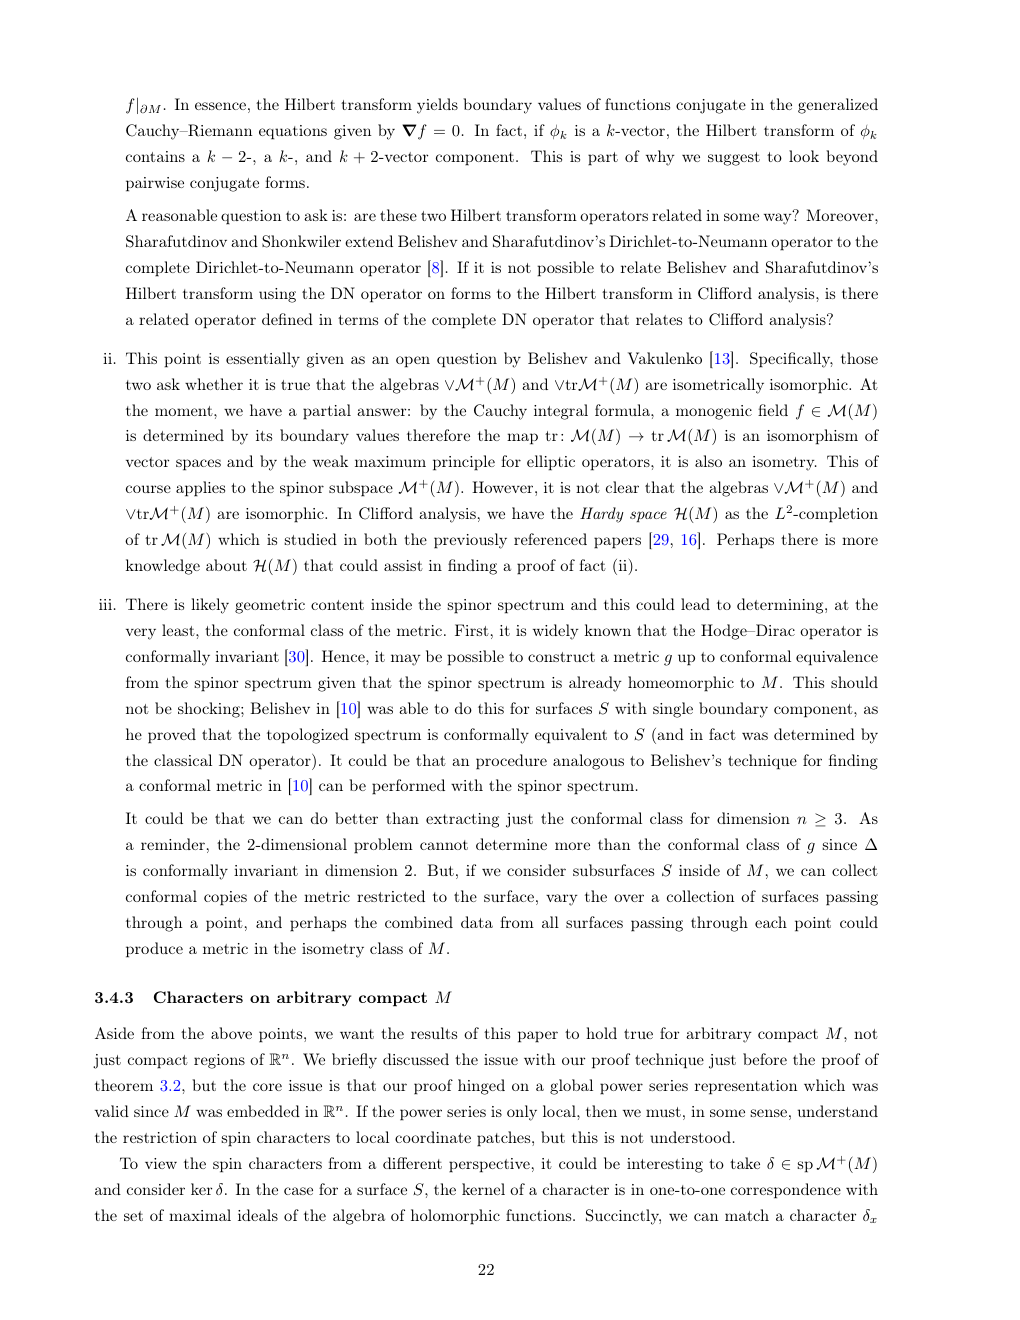
\includegraphics[width=\textwidth,trim=0 540 0 0,clip]{figures/source_page22.png}
\end{center}

Here \(\bigvee\M(M)\) denotes the pointwise algebra generated by the
monogenic even Clifford-valued fields.  We show that, already for the unit
ball \(B^3\), boundary restriction on this algebra has a nontrivial kernel.

\section*{Answer and Proof Intuition}

\begin{theorem}\label{thm:main}
Let \(B^3=\{(x_1,x_2,x_3)\in\mathbb R^3:|x|\leq1\}\), equipped with its
Euclidean metric and positive Clifford convention \(e_i^2=1\).  The boundary
trace homomorphism
\[
 \tr:\bigvee\M(B^3)\longrightarrow
       \bigvee\tr\M(B^3)
\]
is not injective.  In particular, it is neither an algebra isomorphism nor an
isometric isomorphism.
\end{theorem}

The point is that products of monogenic fields need not remain monogenic, and
the generated algebra is consequently much larger than the monogenic space
itself.  Two linear monogenic coordinates already generate the radial
quadratic \(|x|^2\).  Subtracting it from the constant field gives an element
which vanishes on the sphere but not in the ball.

\section*{Proof}

Work in the even Clifford algebra \(\Cl\).  Put
\[
 I=e_1e_2,\qquad J=e_1e_3,\qquad K=e_2e_3.
\]
Then
\[
 I^2=J^2=K^2=-1,\qquad IJ=-K,\qquad IK=J,
 \qquad JK=-I,
\]
with the reversed products having the opposite signs.  Define
\[
 Z=x_2-x_1I,
 \qquad
 W=x_3-x_1J.
\]
For the Euclidean Hodge--Dirac operator
\(D=e_1\partial_{x_1}+e_2\partial_{x_2}+e_3\partial_{x_3}\),
\[
 DZ=e_2-e_1(e_1e_2)=0,
 \qquad
 DW=e_3-e_1(e_1e_3)=0.
\]
Thus \(Z,W\in\M(B^3)\).  Right multiplication by a constant even Clifford
element preserves monogenicity, so all factors below belong to the generating
space used to form \(\A\).

Direct Clifford multiplication gives the identity
\begin{equation}\label{eq:identity}
\begin{split}
 x_1^2+x_2^2+x_3^2
 ={}&Z^2+\frac12ZWK+ZIWJ\\
    &+\frac12WZK-WIWI.
\end{split}
\end{equation}
For completeness, the five terms on the right have components in the ordered
basis \((1,I,J,K)\)
\begin{align*}
Z^2&=(-x_1^2+x_2^2,-2x_1x_2,0,0),\\
\tfrac12ZWK&=(\tfrac12x_1^2,\tfrac12x_1x_2,
              -\tfrac12x_1x_3,\tfrac12x_2x_3),\\
ZIWJ&=(x_1^2,x_1x_2,x_1x_3,-x_2x_3),\\
\tfrac12WZK&=(-\tfrac12x_1^2,\tfrac12x_1x_2,
              -\tfrac12x_1x_3,\tfrac12x_2x_3),\\
-WIWI&=(x_1^2+x_3^2,0,0,0).
\end{align*}
Their non-scalar components cancel, and their scalar components sum to
\(|x|^2\), proving \eqref{eq:identity}.  Every term in its right-hand side is
a finite sum or product of elements of \(\M(B^3)\); hence
\(|x|^2\in\A\).

The constant field \(1\) is monogenic, so
\[
                         P(x)=1-|x|^2
\]
also lies in \(\A\).  Yet \(P|_{\partial B^3}=0\), while \(P(0)=1\).
Therefore \(P\neq0\) belongs to the kernel of the boundary trace
homomorphism.  This proves Theorem \ref{thm:main}. \qed

\section*{Scope, Checks, and Review Focus}

The counterexample addresses exactly the generated-algebra question, not the
paper's separate question about extending its spinor-spectrum theorem to all
compact Riemannian manifolds.  It also explains why the maximum principle for
individual monogenic fields does not pass to their generated algebra: the
kernel element \(1-|x|^2\) is not itself monogenic.

The identity \eqref{eq:identity} was derived by an exact rational linear-algebra
search in the degree-two Clifford polynomial space and then checked by an
independent symbolic expansion retained with this packet.  A bounded novelty
search through August 11, 2026 used the exact paper title, the wording of the
trace-algebra question, and combinations of ``monogenic'', ``boundary trace'',
and ``isometrically isomorphic''; no later primary source giving this negative
answer was found.  Expert review should focus on matching the paper's
\(\bigvee\)-notation with the generated pointwise algebra and on the Clifford
sign convention in \eqref{eq:identity}.

\begin{thebibliography}{9}
\bibitem{Roberts}
C.~Roberts,
\emph{A Gelfand Transform for Spinor Fields on Embedded Riemannian Manifolds},
arXiv:2203.00118v1 (2022), item (ii), p.~22.

\bibitem{BV}
M.~I. Belishev and A.~F. Vakulenko,
\emph{On algebraic and uniqueness properties of 3d harmonic quaternion
fields}, arXiv:1901.09201 (2019).
\end{thebibliography}

\end{document}
